% Session 6 -- ferromagnetic versus antiferromagnetic magnon dispersions, eqs. (6.8) and (6.9).
% Placement: sec. "Magnon dispersions: ferromagnets versus antiferromagnets", after eq. (6.9)
% and the "quadratic in ferromagnets, linear in antiferromagnets" paragraph.
% Rendered by figures/blender/s06f06_dispersion.py, labels in figures/overlays/s06f06_dispersion.tex.
\begin{aqmfigure}{fig:s06:dispersion}{Magnon dispersions (6.8) and (6.9) for a chain ($z=2$,
$\gamma(\mathbf k)=\cos ka$), both in units of $|J|Sz$. Both are zero at $\mathbf k=0$, since a
uniform rotation of all the spins costs no energy. So the magnon is the Goldstone mode of the broken
spin-rotation symmetry, and no value of the exchange can open a gap in it. The difference is
\emph{how} the two dispersions go to zero. The factor $1-\gamma(\mathbf k)$ of the ferromagnet is
quadratic in $k$. The factor $\sqrt{1-\gamma(\mathbf k)^2}$ of the antiferromagnet is the square
root of the same quantity, so it is linear and gives a Dirac-like cone instead of a parabola. The
right panel magnifies the zone centre, where the difference is clear. This extra square root comes
from the Bogoliubov transformation that the N\'eel state requires, since the anomalous $a_ib_j$
terms are what change a parabola into a cone.}
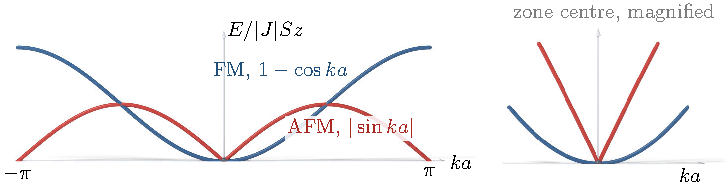
\includegraphics{figures/pdf/s06f06_dispersion.pdf}
\end{aqmfigure}
